\documentclass[border=1pt]{standalone}
\usepackage[T1]{fontenc}
\usepackage{tikz}
\usetikzlibrary{arrows.meta,positioning}
\begin{document}
\begin{minipage}{126mm}
\centering
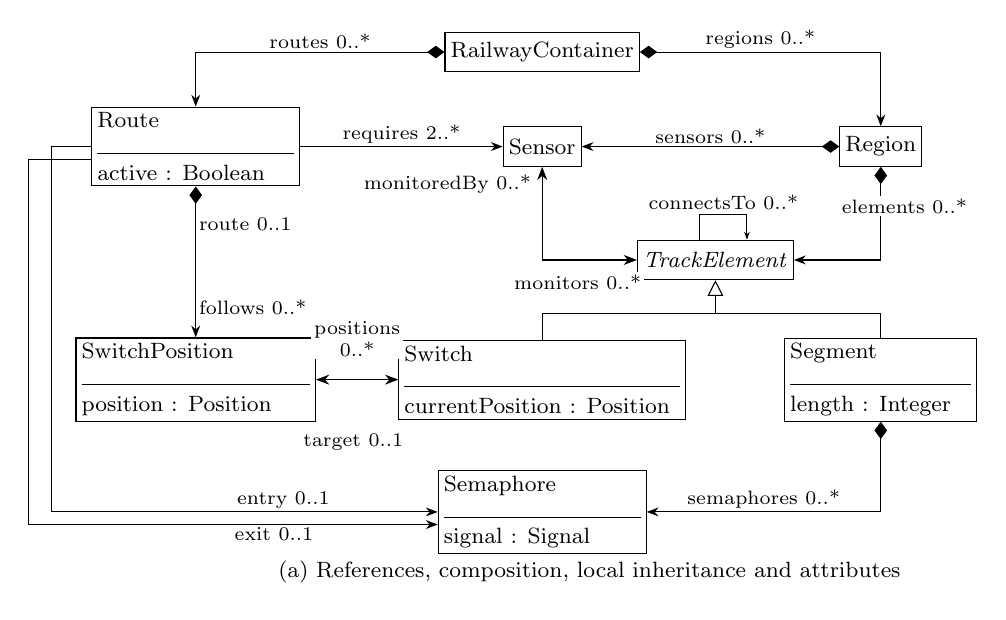
\begin{tikzpicture}[font=\footnotesize,yscale=.8,
 cls/.style={draw,align=center,inner sep=2pt,minimum height=5mm},
 att/.style={cls,align=left},
 lab/.style={font=\scriptsize,fill=white,inner sep=1pt,align=center},
 ref/.style={-{Stealth[length=1.5mm]}},
 comp/.style={{Diamond[length=2.2mm,width=1.6mm]}-{Stealth[length=1.5mm]}},
 inh/.style={-{Triangle[open,length=2mm,width=2mm]}}]
\node[cls] (rc) at (4.4,0) {RailwayContainer};
\node[att] (route) at (0,-1.5) {Route\\\rule{25mm}{.3pt}\\active : Boolean};
\node[cls] (sensor) at (4.4,-1.5) {Sensor};
\node[cls] (region) at (8.7,-1.5) {Region};
\node[cls] (track) at (6.6,-3.3) {\textit{TrackElement}};
\node[att] (pos) at (0,-5.2) {SwitchPosition\\\rule{29mm}{.3pt}\\position : Position};
\node[att] (sw) at (4.4,-5.2) {Switch\\\rule{35mm}{.3pt}\\currentPosition : Position};
\node[att] (seg) at (8.7,-5.2) {Segment\\\rule{23mm}{.3pt}\\length : Integer};
\node[att] (sem) at (4.4,-7.3) {Semaphore\\\rule{25mm}{.3pt}\\signal : Signal};
\draw[comp] (rc.west) -| node[lab,pos=.25,above]{routes 0..*} (route.north);
\draw[comp] (rc.east) -| node[lab,pos=.25,above]{regions 0..*} (region.north);
\draw[comp] (region.west) -- node[lab,above]{sensors 0..*} (sensor.east);
\draw[comp] (region.south) |- (track.east);
\node[lab] at (9,-2.45) {elements 0..*};
\draw[ref] (route.east) -- node[lab,above]{requires 2..*} (sensor.west);
\draw[comp] (route.south) -- node[lab,pos=.25,right]{route 0..1} node[lab,pos=.8,right]{follows 0..*} (pos.north);
\draw[<->,>=Stealth] (sensor.south) |- (track.west);
\node[lab,anchor=east] at (4.3,-2.1) {monitoredBy 0..*};
\node[lab] at (4.85,-3.65) {monitors 0..*};
\draw[-{Stealth[length=1mm,width=.7mm]}]
 ([xshift=-2mm]track.north) -- ++(0,.4) -| ([xshift=4mm]track.north);
\node[lab,anchor=south] at (6.7,-2.55) {connectsTo 0..*};
\coordinate (track-junction) at (6.6,-4.15);
\draw (sw.north) |- (track-junction);
\draw (seg.north) |- (track-junction);
\draw[inh] (track-junction) -- (track.south);
\draw[<->,>=Stealth] (pos.east) -- (sw.west);
\node[lab] at (2.05,-4.55) {positions\\0..*};
\node[lab] at (2,-6.2) {target 0..1};
\draw[comp] (seg.south) |- node[lab,pos=.75,above]{semaphores 0..*} (sem.east);
\draw[ref] (route.west) -- ++(-.5,0) |- node[lab,pos=.8,above]{entry 0..1} (sem.west);
\draw[ref] ([yshift=-2mm]route.west) -- ++(-.8,0) |- node[lab,pos=.8,below]{exit 0..1} ([yshift=-2mm]sem.west);
\node[font=\footnotesize] at (5,-8.25) {(a) References, composition, local inheritance and attributes};
\end{tikzpicture}

\smallskip
\begin{tikzpicture}[font=\footnotesize,yscale=.8,
 cls/.style={draw,align=center,inner sep=2pt,minimum width=24mm},
 inh/.style={-{Triangle[open,length=2mm,width=2mm]}}]
\node[cls] (base) at (0,-1.65) {\textit{RailwayElement}\\\rule{27mm}{.3pt}\\id : Integer};
\node[cls] (r) at (3.5,0) {Region};
\node[cls] (rt) at (3.5,-.66) {Route};
\node[cls] (s) at (3.5,-1.32) {Sensor};
\node[cls] (se) at (3.5,-1.98) {Semaphore};
\node[cls] (sp) at (3.5,-2.64) {SwitchPosition};
\node[cls] (t) at (3.5,-3.3) {\textit{TrackElement}};
\draw (r.west) -- (2,0) -- (2,-3.3) -- (t.west);
\foreach \n in {rt,s,se,sp} \draw (\n.west) -- (2,0 |- \n.west);
\draw[inh] (2,-1.65) -- (base.east);
\node[cls,align=left] at (6.6,-.8) {\textit{\guillemotleft enum\guillemotright}\\Position\\\rule{24mm}{.3pt}\\FAILURE\\STRAIGHT\\DIVERGING};
\node[cls,align=left] at (9.3,-.8) {\textit{\guillemotleft enum\guillemotright}\\Signal\\\rule{24mm}{.3pt}\\FAILURE\\STOP\\GO};
\node[cls,minimum width=20mm] (sw2) at (7,-2.85) {Switch};
\node[cls,minimum width=20mm] (seg2) at (7,-3.6) {Segment};
\draw (sw2.west) -- (5.2,-2.85) -- (5.2,-3.6) -- (seg2.west);
\draw[inh] (5.2,-3.3) -- (t.east);
\node[font=\footnotesize] at (4.5,-4.3) {(b) Inheritance hierarchy and enumerations};
\end{tikzpicture}
\end{minipage}
\end{document}
